\documentclass{report}

\usepackage{hyperref}

\usepackage{epstopdf}
\usepackage{amsmath}
\usepackage{amssymb}
\usepackage{subfig}
%\usepackage{multirow}
\usepackage[utf8]{inputenc}
\usepackage[T1]{fontenc}
\usepackage{standalone}
\usepackage{tikz}
\usepackage{tabularx}
\usepackage{float}
\usepackage[section]{placeins}
\usepackage{sverb}
\usepackage{import}
\usepackage{verbatim}
\usepackage{listings}
\usepackage{xcolor}

\graphicspath{{img/}}
\DeclareGraphicsExtensions{.pdf,.png,.jpg,.svg} %For pdflatex



\begin{document}

\begin{titlepage}
    \begin{center}
        \Huge
        \textbf{Przetwarzanie Obrazów Cyfrowych}
        \\ \vspace{1.5cm}
        \Large
        \textbf{Raport z ćwiczenia 2}        
    \end{center}
    \vspace{4.0cm}
    \Large
    Autor: \\
    Dawid Kania    
\end{titlepage}


\section*{
    Obliczanie liczby barw w obrazie
}
\subsection*{
    Obliczanie liczby barw w obrazie RGB
}




\newcommand{\ww}{0.45} %zmienna używana jako parametr opisujące szerokość obrazu zdefiniowana poraz pierwszy w dokumencie


\begin{figure}[H]
    \captionsetup[subfloat]{justification=raggedright,singlelinecheck=false, position=bottom,labelformat=empty} %
    \subfloat[liczba barw POClab = 54712 \\ liczba barw skrypt = 54712  \\ czas =  1.4128 ]{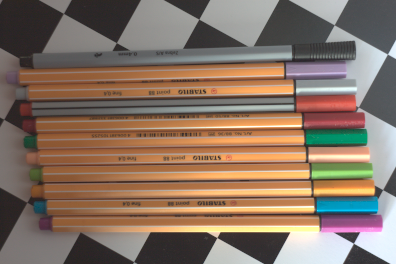
\includegraphics[width=\ww\linewidth]{../obrazy/cienkopisy_srgb.png }} \hfill%	
    \subfloat[liczba barw POClab = 54712 \\ liczba barw skrypt = 54712  \\ czas =  1.4128 ]{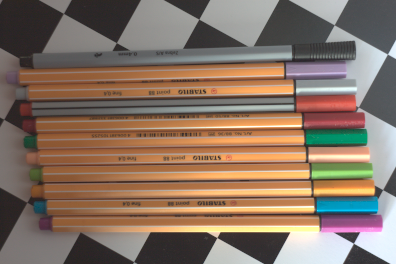
\includegraphics[width=\ww\linewidth]{../obrazy/cienkopisy_srgb.png }} \hfill% wypełnenie
    \caption{tekst to zmiany} 
    \label{fig:porownanie1} %label który można wykorzystać w tekście za pomocą polecenia \ref{fig:porownanie1}
\end{figure}







\newpage

\section*{Kody Programów}


\definecolor{codegreen}{rgb}{0,0.6,0}
\definecolor{codegray}{rgb}{0.5,0.5,0.5}
\definecolor{codepurple}{rgb}{0.58,0,0.82}
\definecolor{backcolour}{rgb}{0.95,0.95,0.92}

\lstdefinestyle{mystyle}{
    backgroundcolor=\color{backcolour},   
    commentstyle=\color{codegreen},
    keywordstyle=\color{magenta},
    numberstyle=\tiny\color{codegray},
    stringstyle=\color{codepurple},
    basicstyle=\ttfamily\footnotesize,
    breakatwhitespace=false,         
    breaklines=true,                 
    captionpos=b,                    
    keepspaces=true,                 
    numbers=left,                    
    numbersep=5pt,                  
    showspaces=false,                
    showstringspaces=false,
    showtabs=false,                  
    tabsize=2
}


\lstset{style=mystyle}

\subsection*{count\_rgb4.m           } \lstinputlisting[language=Octave]{../matlab/count\_rgb4.m         } \newpage
\subsection*{image\_quantization.m   } \lstinputlisting[language=Octave]{../matlab/quantization\_test.m  } \newpage

 





\end{document}